\documentclass[14pt]{extbook}
\usepackage{multicol, enumerate, enumitem, hyperref, color, soul, setspace, parskip, fancyhdr} %General Packages
\usepackage{amssymb, amsthm, amsmath, latexsym, units, mathtools} %Math Packages
\everymath{\displaystyle} %All math in Display Style
% Packages with additional options
\usepackage[headsep=0.5cm,headheight=12pt, left=1 in,right= 1 in,top= 1 in,bottom= 1 in]{geometry}
\usepackage[usenames,dvipsnames]{xcolor}
\usepackage{dashrule}  % Package to use the command below to create lines between items
\newcommand{\litem}[1]{\item#1\hspace*{-1cm}\rule{\textwidth}{0.4pt}}
\pagestyle{fancy}
\lhead{Makeup Progress Quiz 2}
\chead{}
\rhead{Version C}
\lfoot{5763-3522}
\cfoot{}
\rfoot{Spring 2021}
\begin{document}

\begin{enumerate}
\litem{
Choose the graph of the equation below.\[ f(x) = \sqrt{x - 8} + 7 \]\begin{enumerate}[label=\Alph*.]
\begin{multicols}{2}\item 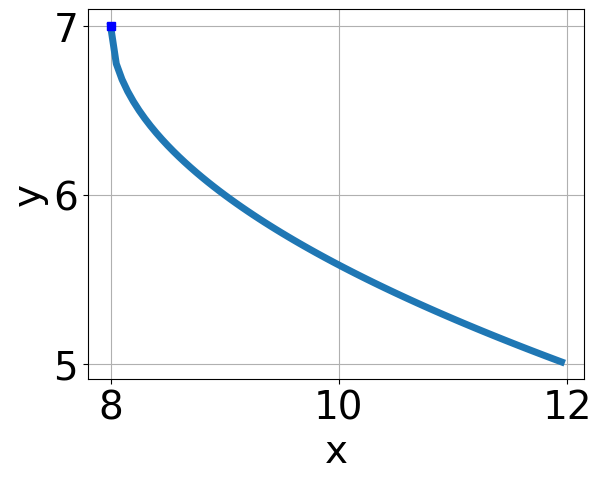
\includegraphics[width = 0.3\textwidth]{../Figures/radicalEquationToGraphAC.png}\item 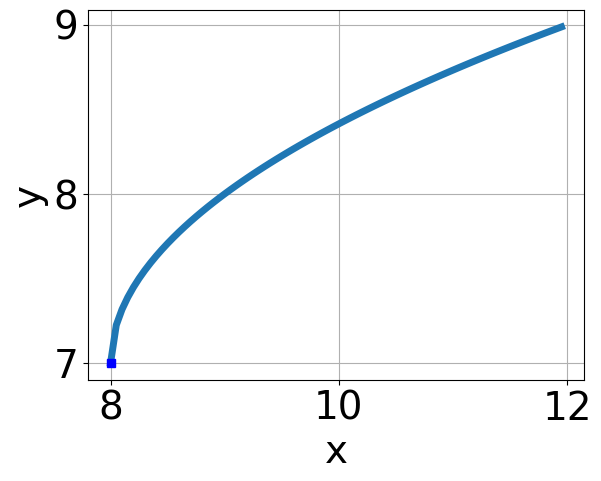
\includegraphics[width = 0.3\textwidth]{../Figures/radicalEquationToGraphBC.png}\item 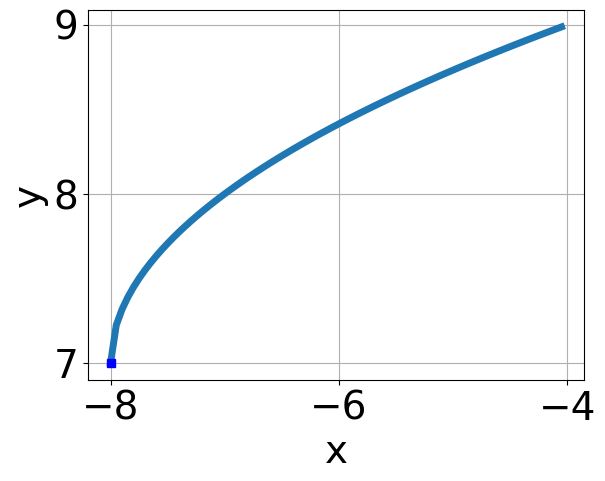
\includegraphics[width = 0.3\textwidth]{../Figures/radicalEquationToGraphCC.png}\item 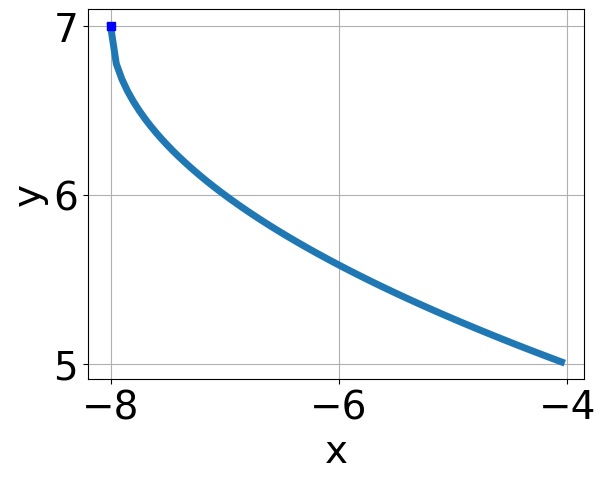
\includegraphics[width = 0.3\textwidth]{../Figures/radicalEquationToGraphDC.png}\end{multicols}\item None of the above.
\end{enumerate} }
\litem{
Choose the equation of the function graphed below.
\begin{center}
    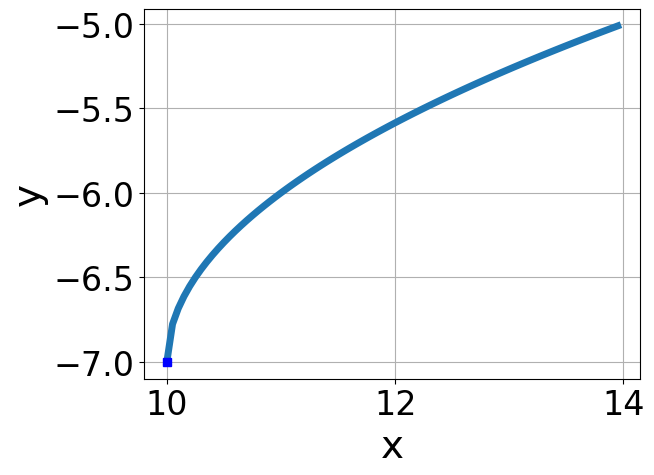
\includegraphics[width=0.5\textwidth]{../Figures/radicalGraphToEquationC.png}
\end{center}
\begin{enumerate}[label=\Alph*.]
\item \( f(x) = - \sqrt{x + 10} - 7 \)
\item \( f(x) = \sqrt{x - 10} - 7 \)
\item \( f(x) = \sqrt{x + 10} - 7 \)
\item \( f(x) = - \sqrt{x - 10} - 7 \)
\item \( \text{None of the above} \)

\end{enumerate} }
\litem{
Choose the graph of the equation below.\[ f(x) = - \sqrt[3]{x + 8} - 5 \]\begin{enumerate}[label=\Alph*.]
\begin{multicols}{2}\item 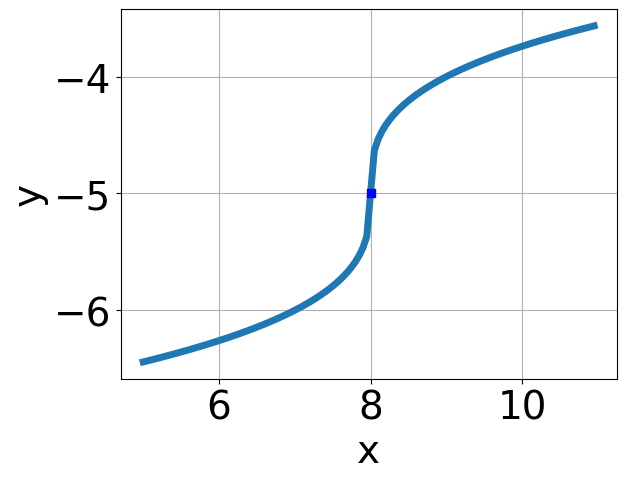
\includegraphics[width = 0.3\textwidth]{../Figures/radicalEquationToGraphCopyAC.png}\item 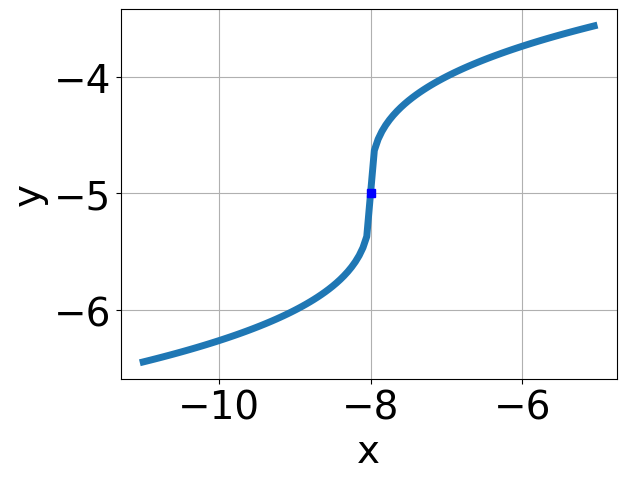
\includegraphics[width = 0.3\textwidth]{../Figures/radicalEquationToGraphCopyBC.png}\item 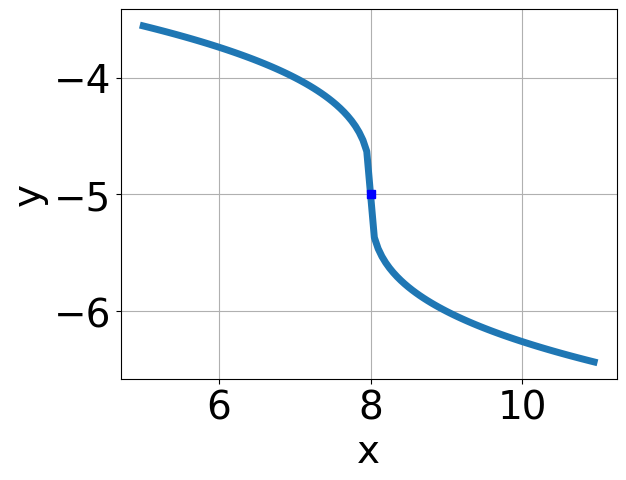
\includegraphics[width = 0.3\textwidth]{../Figures/radicalEquationToGraphCopyCC.png}\item 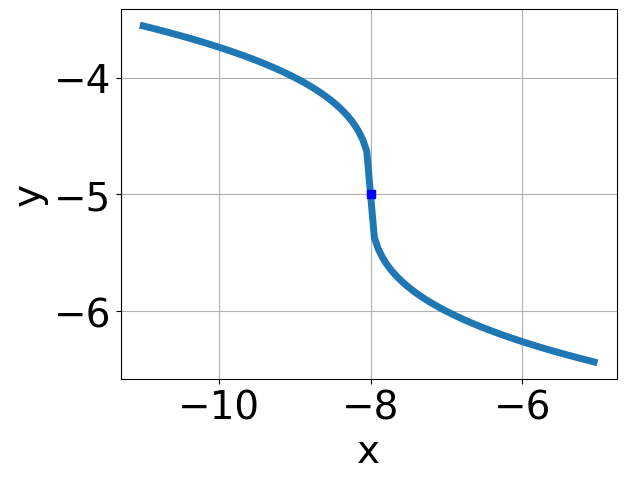
\includegraphics[width = 0.3\textwidth]{../Figures/radicalEquationToGraphCopyDC.png}\end{multicols}\item None of the above.
\end{enumerate} }
\litem{
What is the domain of the function below?\[ f(x) = \sqrt[6]{-3 x - 5} \]\begin{enumerate}[label=\Alph*.]
\item \( [a, \infty), \text{where } a \in [-1.84, -1.44] \)
\item \( (-\infty, \infty) \)
\item \( (-\infty, a], \text{where } a \in [-0.6, 0.4] \)
\item \( (-\infty, a], \text{ where } a \in [-1.67, -0.67] \)
\item \( [a, \infty), \text{where } a \in [-1.32, -0.26] \)

\end{enumerate} }
\litem{
Solve the radical equation below. Then, choose the interval(s) that the solution(s) belongs to.\[ \sqrt{28 x^2 + 24} - \sqrt{-52 x} = 0 \]\begin{enumerate}[label=\Alph*.]
\item \( x \in [-1.03,-0.95] \)
\item \( x_1 \in [0.51, 0.94] \text{ and } x_2 \in [0,2] \)
\item \( \text{All solutions lead to invalid or complex values in the equation.} \)
\item \( x_1 \in [-1.03, -0.95] \text{ and } x_2 \in [-0.86,0.14] \)
\item \( x \in [-0.96,-0.67] \)

\end{enumerate} }
\litem{
What is the domain of the function below?\[ f(x) = \sqrt[3]{5 x + 4} \]\begin{enumerate}[label=\Alph*.]
\item \( (-\infty, \infty) \)
\item \( \text{The domain is } [a, \infty), \text{   where } a \in [-1.05, -0.1] \)
\item \( \text{The domain is } (-\infty, a], \text{   where } a \in [-1.51, -1.1] \)
\item \( \text{The domain is } (-\infty, a], \text{   where } a \in [-0.86, -0.51] \)
\item \( \text{The domain is } [a, \infty), \text{   where } a \in [-1.35, -0.92] \)

\end{enumerate} }
\litem{
Solve the radical equation below. Then, choose the interval(s) that the solution(s) belongs to.\[ \sqrt{-72 x^2 - 27} - \sqrt{99 x} = 0 \]\begin{enumerate}[label=\Alph*.]
\item \( x \in [-2.07,-0.9] \)
\item \( \text{All solutions lead to invalid or complex values in the equation.} \)
\item \( x \in [-0.65,0.87] \)
\item \( x_1 \in [0.44, 1.54] \text{ and } x_2 \in [0.19,0.54] \)
\item \( x_1 \in [-2.07, -0.9] \text{ and } x_2 \in [-1.36,0.23] \)

\end{enumerate} }
\litem{
Solve the radical equation below. Then, choose the interval(s) that the solution(s) belongs to.\[ \sqrt{9 x - 2} - \sqrt{-7 x + 4} = 0 \]\begin{enumerate}[label=\Alph*.]
\item \( x \in [-0.48,0.1] \)
\item \( x \in [0.33,0.48] \)
\item \( x_1 \in [-0.04, 0.27] \text{ and } x_2 \in [0.57,0.64] \)
\item \( x_1 \in [-0.04, 0.27] \text{ and } x_2 \in [0.26,0.4] \)
\item \( \text{All solutions lead to invalid or complex values in the equation.} \)

\end{enumerate} }
\litem{
Solve the radical equation below. Then, choose the interval(s) that the solution(s) belongs to.\[ \sqrt{-5 x - 8} - \sqrt{-7 x + 5} = 0 \]\begin{enumerate}[label=\Alph*.]
\item \( x_1 \in [-5.6, 0.4] \text{ and } x_2 \in [2.5,7.5] \)
\item \( x \in [1.5,2.5] \)
\item \( x \in [3.5,7.5] \)
\item \( x_1 \in [-5.6, 0.4] \text{ and } x_2 \in [-4.29,2.71] \)
\item \( \text{All solutions lead to invalid or complex values in the equation.} \)

\end{enumerate} }
\litem{
Choose the equation of the function graphed below.
\begin{center}
    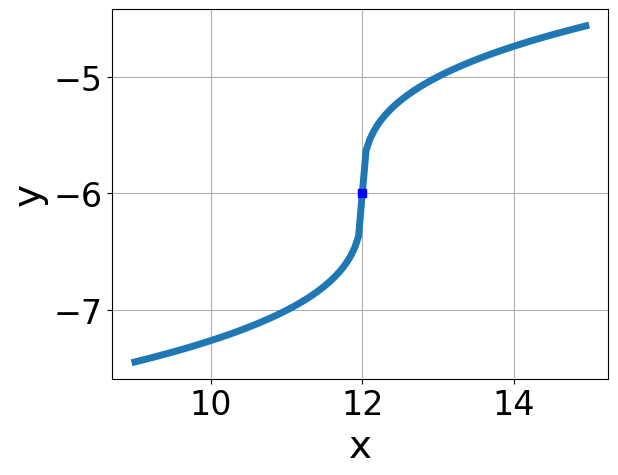
\includegraphics[width=0.5\textwidth]{../Figures/radicalGraphToEquationCopyC.png}
\end{center}
\begin{enumerate}[label=\Alph*.]
\item \( f(x) = - \sqrt{x + 12} - 6 \)
\item \( f(x) = \sqrt{x + 12} - 6 \)
\item \( f(x) = \sqrt{x - 12} - 6 \)
\item \( f(x) = - \sqrt{x - 12} - 6 \)
\item \( \text{None of the above} \)

\end{enumerate} }
\end{enumerate}

\end{document}